\documentclass[11 pt]{article}
\usepackage{structure}

\title{LMECA2660 - Project\\ Simulating 2D flow around an oscillating obstacle}
\author{DEGROOFF Vincent \quad -- \quad NOMA : 09341800}
\date{Friday, 6 may 2022}


\begin{document}

\maketitle

\section{Problem statement}

In this project, we are asked to solve the Navier-Stokes equations for incompressible flows in 2 dimensions, passed a rectangular obstacle. The geometry of the problem is described with more details in figure \ref{fig:domain}.


\begin{figure}[h!tp]
\centering
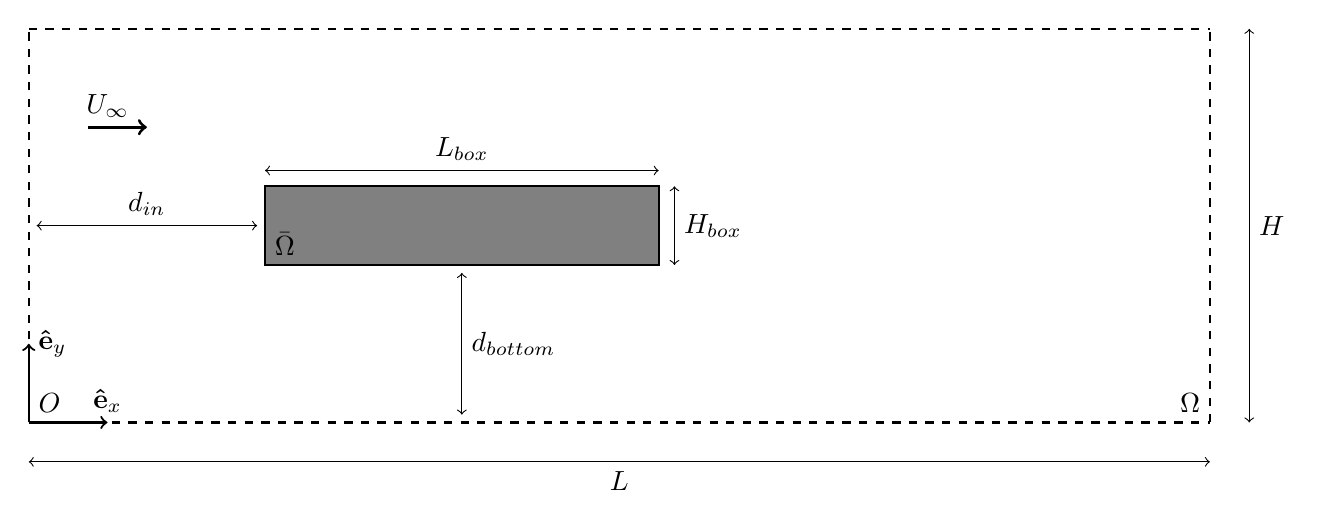
\begin{tikzpicture}[
    every path/.style = {},
    %every node/.append style = {font=\sffamily}
    %every node/.append style = {font=\sffamily}
  ]
  \begin{scope}
    %%+++++++++++++++++++++++++
    % Variables 
    % Box
    \pgfmathsetmacro{\Hbox}{1}
    \pgfmathsetmacro{\Lbox}{5*\Hbox}   
    % Position of the box 
    \pgfmathsetmacro{\xbox}{3*\Hbox}   
    \pgfmathsetmacro{\ybox}{2*\Hbox}   
    % Length of the domain
    \pgfmathsetmacro{\Hdom}{5*\Hbox}
    \pgfmathsetmacro{\Ldom}{15*\Hbox}
    % Length U infinity arrow
    \pgfmathsetmacro{\harr}{0.1*\Hdom}
    %%+++++++++++++++++++++++++
    % Drawing         
     %Domain
    \draw [dashed, thick](0,0) -- (\Ldom,0);
    \draw [dashed, thick](0,\Hdom) -- (\Ldom,\Hdom);
    \draw [dashed, thick](0,0) -- (0,\Hdom);
    \draw [dashed, thick](\Ldom,0) -- (\Ldom,\Hdom);
    \node[above left] at (\Ldom,0){$\Omega$};
    % Flèches:
    \draw[<->] (0,-0.5) -- (\Ldom,-0.5);
    \node[below] at (\Ldom/2,-0.5) {$L$};
    \draw[<->] (\Ldom + 0.5,0) -- (\Ldom + 0.5,\Hdom);
    \node[right] at (\Ldom + 0.5, \Hdom/2) {$H$};
    % Axis 
    \node[above right] at (0,0){$O$};
    \draw[thick, ->] (0,0) -- (1,0);
    \draw[thick, ->] (0,0) -- (0,1);
    \node[rotate=0,above] at (1., 0) {$\mathbf{\hat{e}}_x$};
    \node[rotate=0,right] at (0,1) {$\mathbf{\hat{e}}_y$};
    % Obstacle
    \draw[fill=gray, thick] (\xbox, \ybox) rectangle ++(\Lbox,\Hbox);
    \node[above right] at (\xbox,\ybox){$\bar\Omega$};
    \draw[<->] (0.1, \ybox + 0.5 * \Hbox) -- (\xbox - 0.1, \ybox + 0.5 * \Hbox);
    \node[above] at (\xbox/2, \ybox + 0.5 * \Hbox){$d_{in}$};
    \draw[<->] (\xbox + 0.5 * \Lbox, 0.1) -- (\xbox + 0.5 * \Lbox, \ybox - 0.1);
    \node[right] at (\xbox + 0.5*\Lbox, \ybox/2){$d_{bottom}$};
    \draw[<->] (\xbox, \ybox +  \Hbox + 0.2) -- (\xbox + \Lbox, \ybox +  \Hbox + 0.2);
    \node[above] at (\xbox + 0.5*\Lbox,  \ybox +  \Hbox + 0.2){$L_{box}$};
    \draw[<->] (\xbox + \Lbox + 0.2, \ybox) -- (\xbox + \Lbox + 0.2, \ybox +  \Hbox);
    \node[right] at (\xbox + \Lbox + 0.2,  \ybox +  0.5*\Hbox ){$H_{box}$};
    % U infinity 
    \node[above] at (0.05*\Ldom + 0.25, 0.75*\Hdom){$U_{\infty}$};
    \draw[line width=0.4mm, ->] (0.05*\Ldom, 0.75*\Hdom) -- (0.05*\Ldom + 0.75, 0.75*\Hdom);
    \end{scope}
\end{tikzpicture}
\caption{Description of the case studied. (Image courtesy of Pierre Balty)}
\label{fig:domain}
\end{figure}

In the rest of this document, we will only work with dimensionless variables. Hence, it might be useful to precise the choice of nondimensionalization. Dimensionless quantities are noted here with an asterisk superscript, the position vector is $\mathbf{x} = (x,y)$ and the velocity vector is $\mathbf{v} = (u, v)$.
\begin{equation}
    \begin{split}
        \mathbf{x^*} = \frac{\mathbf{x}}{H_{box}}
    \end{split}
    \qquad
    \begin{split}
        \mathbf{v^*} = \frac{\mathbf{v}}{U_{\infty}}
    \end{split}
    \qquad
    \begin{split}
        t^* = \frac{t U_{\infty}}{H_{box}}
    \end{split}
    \qquad
    \begin{split}
        p^* = \frac{p-p_{ref}}{\rho U_{\infty}^2}
    \end{split}
    \qquad
    \begin{split}
        T^* = \frac{T - T_{ref}}{\Delta T}
    \end{split}
    \label{eq:adimChoice}
\end{equation}

We can also define dimensionless numbers, using physical properties of the fluid: its kinematic viscosity $\nu$, its thermal diffusivity $\alpha$, its heat capacity $c_p$, its density $\rho_0$, and its the volumetric thermal expansion coefficient $\beta=\frac{1}{\rho_0} \left(\pdv{\rho}{T}\right)_p$ where $g$ is the gravitational acceleration.

\begin{equation}
    \begin{split}
        Re = \frac{U_{\infty} H_{box}}{\nu}
    \end{split}
    \qquad
    \begin{split}
        Pr = \frac{\nu}{\alpha}
    \end{split}
    \qquad
    \begin{split}
        Gr = \frac{\beta \Delta T g H_{box}^3}{\nu^2}
    \end{split}
    \qquad
    \begin{split}
        Ec = \frac{U_{\infty}}{c_p \Delta T}
    \end{split}
    \label{eq:adimNumbers}
\end{equation}

\newpage
We can now state the Navier-Stokes equations in dimensionless form, using the Boussinesq approximation. From this point in the document, we will drop this asterisk for the sake of readability.
\begin{align}
    \pdv{u}{x} + \pdv{v}{y} &= 0  && \text{Cons. of mass}\label{eq:nsMass}\\
    \pdv{u}{t} + u\pdv{u}{x} + v\pdv{u}{y} &= -\pdv{p}{x} + \frac{1}{Re} \left( \pdv[2]{u}{x} + \pdv[2]{u}{y} \right) && \text{Cons. of momentum in } \mathbf{\hat e}_{x}\label{eq:nsMomX}\\
    \pdv{v}{t} + u\pdv{v}{x} + v\pdv{v}{y} &= -\pdv{p}{y} + \frac{1}{Re} \left( \pdv[2]{v}{x} + \pdv[2]{v}{y} \right) + \frac{Gr}{Re^2} T && \text{Cons. of momentum in } \mathbf{\hat e}_{y}\label{eq:nsMomY}\\
    \pdv{T}{t} + u\pdv{T}{x} + v\pdv{T}{y} &= \frac{1}{Re \, Pr} \left( \pdv[2]{T}{x} + \pdv[2]{T}{y} \right) + \frac{Ec}{Re} \phi && \text{Cons. of energy} \label{eq:nsEnergy}
\end{align}

Where $\phi$, the viscous dissipation is defined as follows:
\begin{align}
    \phi = 2 \mu \; \mathbf{d:d} = 2 \left[\left(\pdv{u}{x}\right)^2 + \left(\pdv{v}{y} \right)^2\right] + \left(\pdv{u}{y} + \pdv{v}{x}\right)^2 \qquad \text{with} \qquad \mathbf{d} = \frac{1}{2} \left[\left(\nabla u\right) + \left(\nabla u\right)^T \right] \label{eq:dissipation}
\end{align}


\section{Model of the obstacle oscillation}
The rectangular obstacle stays at its initial position in the $x$ direction until a time $t_0$, where its starts oscillating horizontally. The same happens in the $y$ direction, where the threshold time $=\Tilde{t}_0$.

The dimensionless position of the obstacle is then given by:
\begin{equation}
\begin{aligned}
    x_{mesh}(t) - x_{mesh}(t_0) &= \kappa \Big[1 - \cos{\Big(2\pi S_t (t - t_0)\Big)} \Big] && t_0 \leq t\\
    y_{mesh}(t) - y_{mesh}(\tilde t_0) &= \tilde \kappa \Big[1 - \cos{\Big(2\pi \tilde S_t (t - \tilde t_0)\Big)} \Big] && \tilde t_0 \leq t
\end{aligned}
\end{equation}

However, in our model, we need to impose the velocity as boundary condition:
\begin{equation}
\begin{aligned}
    u_{mesh}(t) &= \kappa (2\pi S_t) \sin{\big(2\pi S_t (t - t_0)\big)} = \alpha \sin{\big(2\pi S_t (t - t_0)\big)} && t_0 \leq t\\
    v_{mesh}(t) &= \tilde \kappa (2\pi \tilde S_t ) \sin{\big(2\pi \tilde S_t (t - \tilde t_0)\big)} = \tilde \alpha \sin{\big(2\pi \tilde S_t (t - \tilde t_0)\big)} && \tilde t_0 \leq t
\end{aligned}
\end{equation}

Since the displacement in $\mathbf{\hat e}_y$ is typically used to produce a perturbation, it stops after one period. 

The numerical values chosen for the Strouhal number $S_t$ and the velocity amplitude $\kappa$ are
\begin{equation}
    S_t = \frac{1}{3} \qquad \tilde S_t = S_t \qquad \alpha = \frac{1}{2} \qquad \tilde \alpha = \frac{\alpha}{10}
\end{equation}


\section{Boundary conditions}
(1) The inflow velocity has an horizontal component, with a uniform profile, and no vertical component. (2) The lateral boundaries will be considered as inviscid, with a no-through flow condition and zero vorticity, except stated otherwise. (3) No-through flow and no-slip conditions are enforced at the obstacle boundaries. (4) At the outflow, we try to mimic a transparent boundary condition, by advecting the fields $u$, $\omega$ and $T$ at a velocity $u_c = 1-u_{mesh}$. (5) Except at the outflow, the boundary conditions for temperature will be either adiabatic or Dirichlet. To be more precise, a summary of these boundary conditions is presented in table \ref{tab:boundary}.
\begin{table}[H]
    \centering
    \begin{tabularx}{\textwidth}{@{\extracolsep{\stretch{1}}}*{4}{c}@{}}
    \toprule
    Location & First condition & Second condition & Temperature condition\\
    \midrule
    Inflow & $u=1$ & $v=0$ & $\pdv{T}{x} = 0$\\[8pt]
    Lateral walls & $u=1$ (or $u=0$) & $v=0$ & $\pdv{T}{y} = 0\;$ or $\;T=T_{wall}$\\[8pt]
    Obstacle wall & $u=0$ & $v=0$ & $\pdv{T}{n} = 0\;$ or $\;T=T_{wall}$\\[8pt]
    Outflow & $\pdv{u}{t} + u_c \pdv{u}{x} = 0$ & $\pdv{\omega}{t} + u_c \pdv{\omega}{x} = 0$ & $\pdv{T}{t} + u_c \pdv{T}{x} = 0$ \\
    \bottomrule
    \end{tabularx}
    \caption{Boundary conditions of the dimensionless fields.}
    \label{tab:boundary}
\end{table}

\section{Numerical solver}
The Navier-stokes equations shown in \eqref{eq:nsMass}-\eqref{eq:nsEnergy} are integrated in time using a two-step projection scheme that ensures a divergence-free velocity field $\bv$. The fields $u$, $v$, $p$, $\omega$ and $T$ are discretized using the staggered MAC mesh which is represented in figure \ref{fig:macMesh}. In this project, we use a uniform grid with $\Delta x = \Delta y = h$, but a non-uniform grid with stretching would be more adapted. It would allow us to have a coarser mesh where nothing happens (outside the boundary layer and outside the vortex shedding).

When a boundary condition must be applied at some position $\mathbf{x}$ where a field is not defined, we define \textit{ghost points} outside the domain that approximate the condition using Taylor series.

\begin{figure}[H]
    \centering
    \includesvg[width=\textwidth]{../figures/mac_mesh.svg}
    \caption{Staggered MAC mesh near a rectangular corner of the domain $\Omega$. Ghost points are more transparent than regular points.}
    \label{fig:macMesh}
\end{figure}


Concerning the time integration, the convective term is integrated using the explicit and second order Adams-Bashforth scheme (explicit Euler scheme for the first time step), while the diffusive term is handled using the explicit and first order Euler scheme. The solver proposed can also handle the diffusive term for $\bv$ with a Crank-Nicolson scheme. This is done with an ADI method in order to only solve tri-diagonal systems. However, the current implementation of boundary conditions is not assured to be second order.

First, we compute the convective terms $\bH = (H_x, H_y)$ that discretize $(\boldsymbol\nabla \bv) \cdot (\bv - \bv_{mesh})$, and $H_T$ discretizing $(\boldsymbol \nabla T) \cdot (\bv - \bv_{mesh})$. Second, we perform a predictor step to obtain an intermediate field denoted $\mathbf{v}^*$. Third, we solve the Poisson equation for $\Phi$, using the PETSC library \cite{petsc-efficient}. 
Finally, we obtain the next iterates once the corrector step is completed. This procedure is detailed in equations \eqref{eq:predictor} - \eqref{eq:corrector}.

\begin{align}
    \frac{\bv^* - \bv^n}{\Delta t} &= \frac{-1}{2} \left(3\,\bH^n - \bH^{n-1}\right) - \boldsymbol{\nabla} p^n + \frac{1}{Re} \nabla^2 \bv^n - \frac{Gr}{Re^2} \frac{\mathbf{g}}{\left\|\mathbf{g}\right\|} T^n \label{eq:predictor} \\[10pt]
    \nabla^2\Phi &= \frac{1}{\Delta t} \; \nabla \cdot \bv^*\\[10pt]
    \frac{\bv^{n+1} - \bv^*}{\Delta t} &= -\boldsymbol{\nabla} \Phi\\[10pt]
    p^{n+1} &= p^n + \Phi\\[10pt]
    T^{n+1} &= \frac{-1}{2} \left(3\, H_T^n - H_T^{n-1}\right) + \frac{1}{Re\, Pr} \nabla^2 T^n + \frac{Ec}{Re} \phi^n \label{eq:corrector}
\end{align}

The convection contribution can be computed using either the advective form or the divergence form, respectively:
\begin{equation}
    \bH = (\boldsymbol\nabla \bv) \cdot (\bv - \bv_{mesh}) \qquad \text{or} \qquad \bH = \boldsymbol\nabla \cdot \big(\bv \, (\bv - \bv_{mesh}) \big)
\end{equation}
It was chosen to take the average of both.

To ensure the stability of the scheme, the \textit{Fourier number} and the \textit{Courant-Friedrichs-Lewy number} were respectively set to \footnote{Recall that the variables $\Delta t$, $h$, $u$ and $v$ are dimensionless, so that $r$ and $CFL$ are also.}
\begin{equation}
    r = \frac{\Delta t}{Re \, h^2} = 0.2 \qquad\qquad CFL = \frac{(|u|+|v|) \Delta t}{h} = 0.7
\end{equation}
where the velocity $(|u|+|v|)$ was estimated to $4$. As an option, the program can use an adaptive time step $\Delta t$ based on the velocity maximum value of $|u|+|v|$ computed at the previous step.


\section{Simulations without temperature coupling}
Different cases will be considered:
\begin{enumerate}[topsep=0pt]
    \setlength\itemsep{0pt}
    \item The obstacle stays at rest. The flow is steady, but unstable.
    \item The obstacle oscillates vertically during one period, starting at $\tilde t_0 = 0$, to break the symmetry and obtain an unsteady flow.
    \item The obstacle oscillates horizontally, starting at $t_0=0$.
    \item The obstacle oscillates horizontally, starting at $t_0=0$. But we also add a vertical perturbation of one period, starting at $\tilde t_0=0$ to initiate an asymmetrical vortex shedding.
    %\item The obstacle oscillates vertically, starting at $\tilde t_0=0$. In order to have a smoother simulation, the amplitude of the sine wave is progressively increased from $0$ to $\tilde \kappa$ over multiple periods.
\end{enumerate}

Based on the simulation of each of these cases, some analysis and visualizations will be provided: the vorticity field $\omega$, the streamfunction $\psi$ with its associated streamlines, the drag coefficient $C_d$, the lift coefficient $C_l$ and the evolution of the mesh Reynolds number indicating the quality of the simulation.

With the expression of the vorticity in 2D
\begin{equation}
    \omega = \nabla \times \mathbf{v} = \pdv{v}{x} - \pdv{u}{y}
\end{equation}
we can easily computed $\omega$ on the staggered grid as shown previously in figure \ref{fig:macMesh}, using centered finited differences.

The streamfunction is defined by
\begin{equation}
    u = -\pdv{\psi}{y} \qquad v = \pdv{\psi}{x}
\end{equation}
The value $\psi(x,y)$ can therefore be computed over the whole domain $\Omega$ by integrating the differential form $d\psi = v \diff x -u \diff y = \mathbf{v} \cdot \mathbf{\hat n} \diff s$ along some path $\Gamma$ from the reference point $(0,0)$ to $(x,y)$. We should note that the result is path-independent since the flow is diveregence-free. In fact, if one choses another path $\Gamma'$ from $(0,0)$ to $(x,y)$, we can obtain a closed curve $C$ by concatenating both curves:
\begin{equation}
    \int_{\Gamma} \mathbf{v} \cdot \mathbf{\hat n} \diff s + \int_{-\Gamma'} \mathbf{v} \cdot \mathbf{\hat n} \diff s = \oint_{C} \mathbf{v} \cdot \mathbf{\hat n} \diff s = \iint_{S} \nabla \cdot \mathbf{v} \diff a = 0
\end{equation}

The drag force $D$ and the lift force $L$ can be computed by integrating the stress tensor $\boldsymbol \sigma$ on the boundary $\partial \bar \Omega$ of the rectangular body $\bar \Omega$. With dimensional variables, we have

\begin{equation}
    \mathbf{F} = D \,\mathbf{\hat{e}}_x + L \,\mathbf{\hat{e}}_y = \int_{\partial \bar \Omega} \mathbf{n} \cdot \boldsymbol \sigma = \int_{\partial \bar \Omega} \mathbf{n} \cdot (-p \boldsymbol \delta + 2 \mu \mathbf{d})
\end{equation}

After some simplifications, and a nondimensionalization, we obtain
\begin{align}
    C_d = \frac{D}{\frac{1}{2} \rho U_{\infty}^2} &= \bigintss_{y^-}^{y^+} \Big[p(x^-, y) - p(x^+, y)\Big] \diff y + \frac{1}{Re} \bigintss_{x^-}^{x^+} \left[ \left.\pdv{u}{y}\right|_{(x, y^+)} - \left.\pdv{u}{y}\right|_{(x, y^-)} \right] \diff x\\
    C_l = \frac{L}{\frac{1}{2} \rho U_{\infty}^2} &= \bigintss_{x^-}^{x^+} \Big[p(x, y^-) - p(x, y^+)\Big] \diff x + \frac{1}{Re} \bigintss_{y^-}^{y^+} \left[ \left.\pdv{v}{x}\right|_{(x^+, y)} - \left.\pdv{v}{x}\right|_{(x^-, y)} \right] \diff y
\end{align}
where $x^-$ and $x^+$ respecitvely refer to the $x$ value on the left and right sides of the rectangle, and $y^-$ and $y^+$ respecitvely refer to the $y$ value on the bottom and the top of the rectangle.

Finally, two mesh Reynolds numbers can be computed:
\begin{align}
    Re_h &= (|u|+|v|) \,h \, Re && \text{based on the velocity of the flow}\\
    Re_{\omega} &= |\omega| \,h^2 \, Re && \text{based on the vorticity of the flow}
\end{align}
Here, we are only interrested about their maximum value over the domain $\Omega$ at each time step.


%%%%%%%%%%%%%%%%%%%%%%%%%%%%%%%%%%%%%%%%%%%%%%%%%%%%%%%%%%%%%%%%%%%%%%%%%%%%%%%%%

\subsection{Case 1: obstacle at rest with symmetrical flow}

\begin{figure}[H]
    \centering
    \includesvg[width=\textwidth]{../figures/vorticity_case_1.svg}
    \caption{Level sets of the vorticity $\omega$ in \textit{case 1} at different dimensionless times $t$. These levels sets are slightly more concentrated around zero for a better visualization.}
    \label{fig:vorticity_1}
\end{figure}

A few remarks:
\begin{itemize}
    \item The vorticity is the highest around the left corners of the obstacle, near the inflow.
    \item There are two kind of recirculation regions: the first kind above and below the rectangle, and the second kind behind.
    \item The flow rotates clockwise ($\omega < 0$) in the boundary layer located above the obstacle, except very near the wall ($\omega > 0$), and reciprocally below the obstacle.
\end{itemize}

\begin{figure}[H]
    \centering
    \includesvg[width=\textwidth]{../figures/streamlines_case_1.svg}
    \caption{Snapshot of the streamlines of \textit{case 1}. The color is proportional to the velocity norm. The width of the lines is proportional to $\left|1 - \|\mathbf{v}\|\right|$ in order to highlight the regions where $\mathbf{v}$ is very different than the mean-flow.}
    \label{fig:streamlines_1}
\end{figure}
As show, in figure \ref{fig:streamlines_1}, the recirculation region grows with time. The stagnation point moves from $x-x_{wall} \approx 3$ at $t=12.5$ to $x - x_{wall} \approx 4.5$ at $t=25.$. The flow recirculation even becomes too large for the computational domain since the stagnation point grows beyond $x=15$ at $t \approx 40$.

The mesh Reynolds numbers are shown in figure \ref{fig:mesh_re_case1}. Their value quickly decrease before stabilizing around $25$. This is due to the fact that the flow is initially unphysical with discontinuities of $u$ near the walls that degrade the numerical solutions.

In figure \ref{fig:drag_case1}, as expected the lift is zero (or almost due to numerical rounding errors) since the flow is symmetrical. On the other hand, the drag coefficient is non-zero, and $C_d \approx 1.25$ while the stagnation point stays inside the domain.

\begin{figure}[H]
    \centering
    \includesvg[width=\textwidth]{../figures/mesh_Re_case_1.svg}
    \caption{Mesh Reynolds numbers evolution for \textit{case 1}.}
    \label{fig:mesh_re_case1}
\end{figure}


\begin{figure}[H]
    \centering
    \includesvg[width=0.95\textwidth]{../figures//drag_lift_case_1.svg}
    \caption{Aerodynamic coefficients evolution for \textit{case 1}.}
    \label{fig:drag_case1}
\end{figure}



%%%%%%%%%%%%%%%%%%%%%%%%%%%%%%%%%%%%%%%%%%%%%%%%%%%%%%%%%%%%%%%%%%%%%%%%%%%%%%%%%

\subsection{Case 2: obstacle at rest with unsymmetrical flow}
\begin{figure}[H]
    \centering
    \includesvg[width=\textwidth]{../figures/vorticity_case_2.svg}
    \caption{Level sets of the vorticity $\omega$ in \textit{case 2} at different dimensionless times $t$.}
    \label{fig:vorticity_2}
\end{figure}

Now, the flow is unsteady, but becomes periodic around $t=10$. In this configuration, positive and negative vortices detach one after the other. In figure \ref{fig:vorticity_2}, we can observe a vortex, in blue above the rectangle detaching from the boundary layer. The half-period $T/2$, or delay between the ejection of a "positive" vortex ($\omega$ > 0) and a "negative" vortex ($\omega$ < 0) and  appears to last approximately $2$ to $3$ dimensionless times.

\begin{figure}[H]
    \centering
    \includesvg[width=\textwidth]{../figures/streamlines_case_2.svg}
    \caption{Streamlines of the flow in case 2 at different dimensionless times $t$. }
    \label{fig:streamlines_2}
\end{figure}

In figure \ref{fig:streamlines_2}, we observe many small recirculation regions near the obstacle walls. If we move away a little bit more from the upper and lower walls of the rectangle, we observe that the flow accelerates around the obstacle: this remark holds for all the cases.


\begin{figure}[H]
    \centering
    \includesvg[width=\textwidth]{../figures/avg_flow_case_2.svg}
    \caption{Streamlines and vorticity of the average of flow of \textit{case 2} from $t=20$ to $t=60$.}
    \label{fig:averaging_2}
\end{figure}

Looking the averaged-time flow in \ref{fig:averaging_2}, we observe that the recirculation region is much smaller than in \textit{case 1}: the \textit{averaged stagnation point} is located $\approx 1$ dimensionless unit behind the rectangle.

The mesh Reynolds number also oscillates with the vortex shedding as shown in figure \ref{fig:mesh_re_case2}, with this half-period $T/2$.

In figure \ref{fig:mesh_re_case2}, the drag coefficient $C_d$ oscillates as well with that period $T/2$, while the lift coefficient oscillates with the full period $T$. This is because the vortices rotate alternatively clockwise and anticlockwise.

Remark: the time axis of the aerodynamic coefficients stops at $t=50$ and not $t=60$ for a better visualization, but the flow was computed until $t=60$.

\begin{figure}[H]
    \centering
    \includesvg[width=\textwidth]{../figures/mesh_Re_case_2.svg}
    \caption{Mesh Reynolds numbers evolution for \textit{case 2}.}
    \label{fig:mesh_re_case2}
\end{figure}

\begin{figure}[H]
    \centering
    \includesvg[width=0.95\textwidth]{../figures//drag_lift_case_2.svg}
    \caption{Aerodynamic coefficients evolution for \textit{case 2}.}
    \label{fig:drag_case2}
\end{figure}

%%%%%%%%%%%%%%%%%%%%%%%%%%%%%%%%%%%%%%%%%%%%%%%%%%%%%%%%%%%%%%%%%%%%%%%%%%%%%%%%%

\subsection{Case 3: obstacle oscillating with symmetrical flow}

\begin{figure}[H]
    \centering
    \includesvg[width=\textwidth]{../figures/vorticity_case_3.svg}
    \caption{Level sets of the vorticity $\omega$ in \textit{case 3} at different dimensionless times $t$.}
    \label{fig:vorticity_3}
\end{figure}
%Now, the rectangle oscillates horizontally with a period $\Delta t = 1/S_t = 3$.

The vorticity levels are shown in \ref{fig:vorticity_3}, at different times covering an oscillation period of the rectangle:
\begin{itemize}
    \item at $t=42$, the obstacle is at it leftmost position with maximum velocity headed to the right.
    \item at $t=43$, the obstacle has almost reached its rightmost position, still moving to the right, but slowing down.
    \item at $t=44$, the obstacle is now moving to left, reaching the same position as at $t=43$.
\end{itemize}

Vortices are generated around the upper left and lower left corners of the obstacle at $t=0 \: \textrm{mod} \: 3$, before \textit{sliding} close to the wall and finally detaching.

Two remarks about figure \ref{fig:drag_case4}:
\begin{itemize}
    \item The lift coefficient $C_l$ is again zero since the flow is symmetrical, as in \textit{case 1}.
    \item The drag coefficient can become negative: when the box is accelerating to the right, the fluid resists this motion and \textit{pushes} the box to the left.
\end{itemize}

\begin{figure}[H]
    \centering
    \includesvg[width=\textwidth]{../figures/mesh_Re_case_3.svg}
    \caption{Mesh Reynolds numbers evolution for \textit{case 3}.}
    \label{fig:mesh_re_case3}
\end{figure}


\begin{figure}[H]
    \centering
    \includesvg[width=0.95\textwidth]{../figures/drag_lift_case_3.svg}
    \caption{Aerodynamic coefficients evolution for \textit{case 3}.}
    \label{fig:drag_case3}
\end{figure}

%%%%%%%%%%%%%%%%%%%%%%%%%%%%%%%%%%%%%%%%%%%%%%%%%%%%%%%%%%%%%%%%%%%%%%%%%%%%%%%%%

\subsection{Case 4: obstacle oscillating with unsymmetrical flow}

\begin{figure}[H]
    \centering
    \includesvg[width=\textwidth]{../figures/vorticity_case_4_part1.svg}
    \caption{Level sets of the vorticity $\omega$ in \textit{case 4} at different dimensionless times $t$.}
    \label{fig:vorticity_4a}
\end{figure}

Now, thanks to the vertical perturbation, we obtain a non-symmetrical vortex shedding. In figure \ref{fig:vorticity_4a}, the vorticity field is shown at the same times as for \textit{case 3} - figure \ref{fig:vorticity_3}. As opposed to the \textit{case 2}, we see that the vortices come by pair: one generated upstream due to the friction along the wall, the other one generated downstream behind the obstacle. 

\begin{figure}[H]
    \centering
    \includesvg[width=\textwidth]{../figures/vorticity_case_4_part2.svg}
    \caption{Level sets of the vorticity $\omega$ in \textit{case 4} at different dimensionless times $t$ - continued.}
    \label{fig:vorticity_4b}
\end{figure}

In figure \ref{fig:vorticity_4b}, the field is shown for three more dimensionless times $t=45,\, 46,\, 47$. This shows that the period of the vortex shedding is twice the period of the rectangle oscillation.

\begin{figure}[H]
    \centering
    \includesvg[width=\textwidth]{../figures/mesh_Re_case_4.svg}
    \caption{Mesh Reynolds numbers evolution for \textit{case 3}.}
    \label{fig:mesh_re_case4}
\end{figure}

\begin{figure}[H]
    \centering
    \includesvg[width=0.95\textwidth]{../figures//drag_lift_case_4.svg}
    \caption{Aerodynamic coefficients evolution for \textit{case 4}.}
    \label{fig:drag_case4}
\end{figure}

% \begin{figure}[H]
%     \centering
%     \includesvg[width=\textwidth]{../figures/vorticity_vertical.svg}
%     \caption{Level sets of the vorticity $\omega$ in \textit{case 5} at different dimensionless times $t$.}
%     \label{fig:vorticity_5}
% \end{figure}

% \begin{figure}[H]
%     \centering
%     \includesvg[width=\textwidth]{../figures/avg_flow_case_3.svg}
%     \caption{Averaging of case 3 from $t=20$ to $t=60$.}
%     \label{fig:averaging_3}
% \end{figure}

% \begin{figure}[H]
%     \centering
%     \includesvg[width=\textwidth]{../figures/avg_flow_case_4.svg}
%     \caption{Averaging of case 4 from $t=20$ to $t=60$.}
%     \label{fig:averaging_4}
% \end{figure}

% \begin{figure}[H]
%     \centering
%     \includesvg[width=\textwidth]{../figures/avg_flow_vertical.svg}
%     \caption{Averaging of case 5 from $t=20$ to $t=60$.}
%     \label{fig:averaging_5}
% \end{figure}


\section{Simulations with temperature coupling}

\subsection{Hot obstacle}

\subsection{Obstacle cold above and hot underneath}

\subsection{No-slip walls with fixed temperature}

\subsection{Heat generation through viscous dissipation}

\newpage


% 
% \printbibliography

\bibliographystyle{plain}
\nocite{*}
\bibliography{main.bib}

\end{document}
